\documentclass{sciposter}
\usepackage{lipsum}
\usepackage{epsfig}
\usepackage{amsmath}
\usepackage{amssymb}
\usepackage{multicol}
\usepackage{graphicx,url}
\usepackage{textpos}   
\usepackage[utf8]{inputenc}
\usepackage{xcolor}
\usepackage{tabularx}
\newtheorem{Def}{Definition}



\title{
\leavevmode{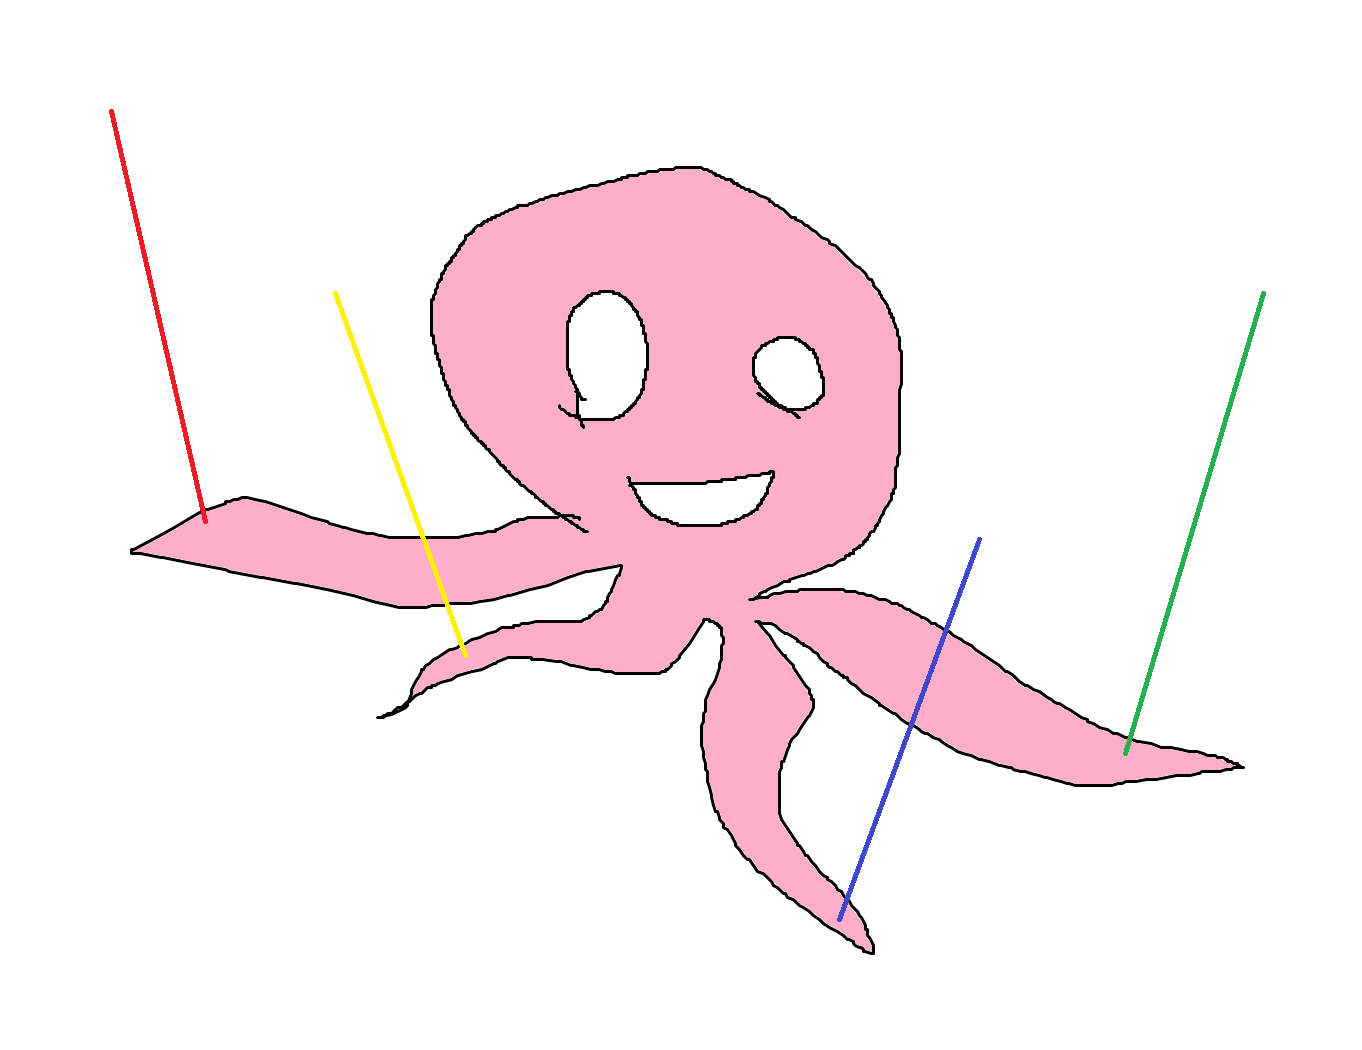
\includegraphics[width=0.3\textwidth]{Logos/gestikulaser.png}}\\
Gestikulaser}
%Título do projeto

\author{Christoph Behr, Cailing Fu, Nicole Grubert, Daniel Wolff}
%nome dos autores by the current \maketitle

%\renewcommand\printleftlogo
%  {\begin{center}
%     \resizebox{\textwidth}{!}%
%       {
\includegraphics{TOSLogo.png}
\includegraphics{COSIMALogo.png}}
%   \end{center}
%  }
  
%\rightlogo[2]{TOSLogo.png}
%\leftlogo[2]{COSIMALogo}

%Section title color:
\definecolor{SectionCol}{rgb}{0.0, 0.329411, 0.62353} % RWTH Blau
% Section block color:
\definecolor{BoxCol}{rgb}{0.949,0.949,0.949} % Grau

\begin{document}

% TOS Logo oben links
\begin{textblock*}{60px}(0cm,0cm)

\includegraphics[height=6cm,width=20cm]{Logos/TOS.png}
\end{textblock*}

% COSIMA18 Logo oben rechts
\begin{textblock*}{60px}(55cm,0mm)

\includegraphics[height=6cm,width=20cm]{Logos/Cosima18.png}
\end{textblock*}

\maketitle

%%% Begin of Multicols-Enviroment
\begin{multicols}{3}
\setlength{\parindent}{2em}

\section{Unsere Vision}
Gestenerkennung ist immer wieder ein Thema, welches viel Aufmerksamkeit erregt. Und obwohl der Mensch so einfach typische Gesten erkennen kann, bleibt es für den Computer eine große Herausforderung, zuverlässig die Gesten eines Menschen zuzuordnen. \\
Mit Gestikulaser wollen wir ein neues System entwickeln, um die Handgesten eines Menschen zu erkennen und diese individuell auf den Nutzer ab zu stimmen. Dabei soll es nicht, wie die meisten heute typischen Systeme, mit einer Kamera arbeiten, sondern durch Lichtreflexionen einer Hand die Geste zuordnen. Denn damit ist die Gestenerkennung nicht nur Tageslicht unabhängig, sondern kann auch in vollkommener Dunkelheit betrieben werden. \\

\section{Der Gestikulaser}
Der Gestikulaser besteht aus zwei Teilen, einer Photoplatte sowie einer Machine Learning Software. \\
Die Photoplatte ist ausgestattet mit mehreren infrarot LED Quellen, sowie einer Vielzahl von Photodioden, welche ausschließlich infrarotes Licht detektiert. Durch die Lichtreflexion der Hand oberhalb der Photoplatte können verschiedene Intensitäten an den Photodioden gemessen werden. Durch diese Intensitäten soll dann mit Hilfe der Machine Learning Software eine eindeutige Geste erkannt werden. Diese Geste kann dazu genutzt werden verschiedene Dinge wie ein Auto oder eine Smart Home Einrichtung zu steuern.\\

\begin{figure}[h]
	\centering
	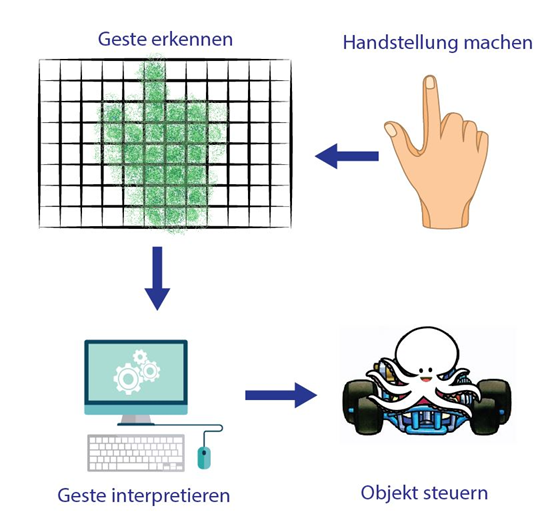
\includegraphics[scale=1.3]{figures/AblaufGestikulaser.png}
	\caption{Schematischer Ablauf von einer Handgeste zu einer Objektsteuerung}
	\label{fig:Sensorhandschuh}
\end{figure}

\section{Die Beta-Version}
Während unserer Konstruktion des Gestikulasers erstellten wir eine vorläufige Photoplatte, welche fix angebrachte Photodioden auf der Oberseite der Photoplatte hatte. Damit konnte gezeigt werden: unsere Idee funktioniert. Verschiedene Gesten konnten erkannt werden!

\begin{figure}[h]
	\centering
	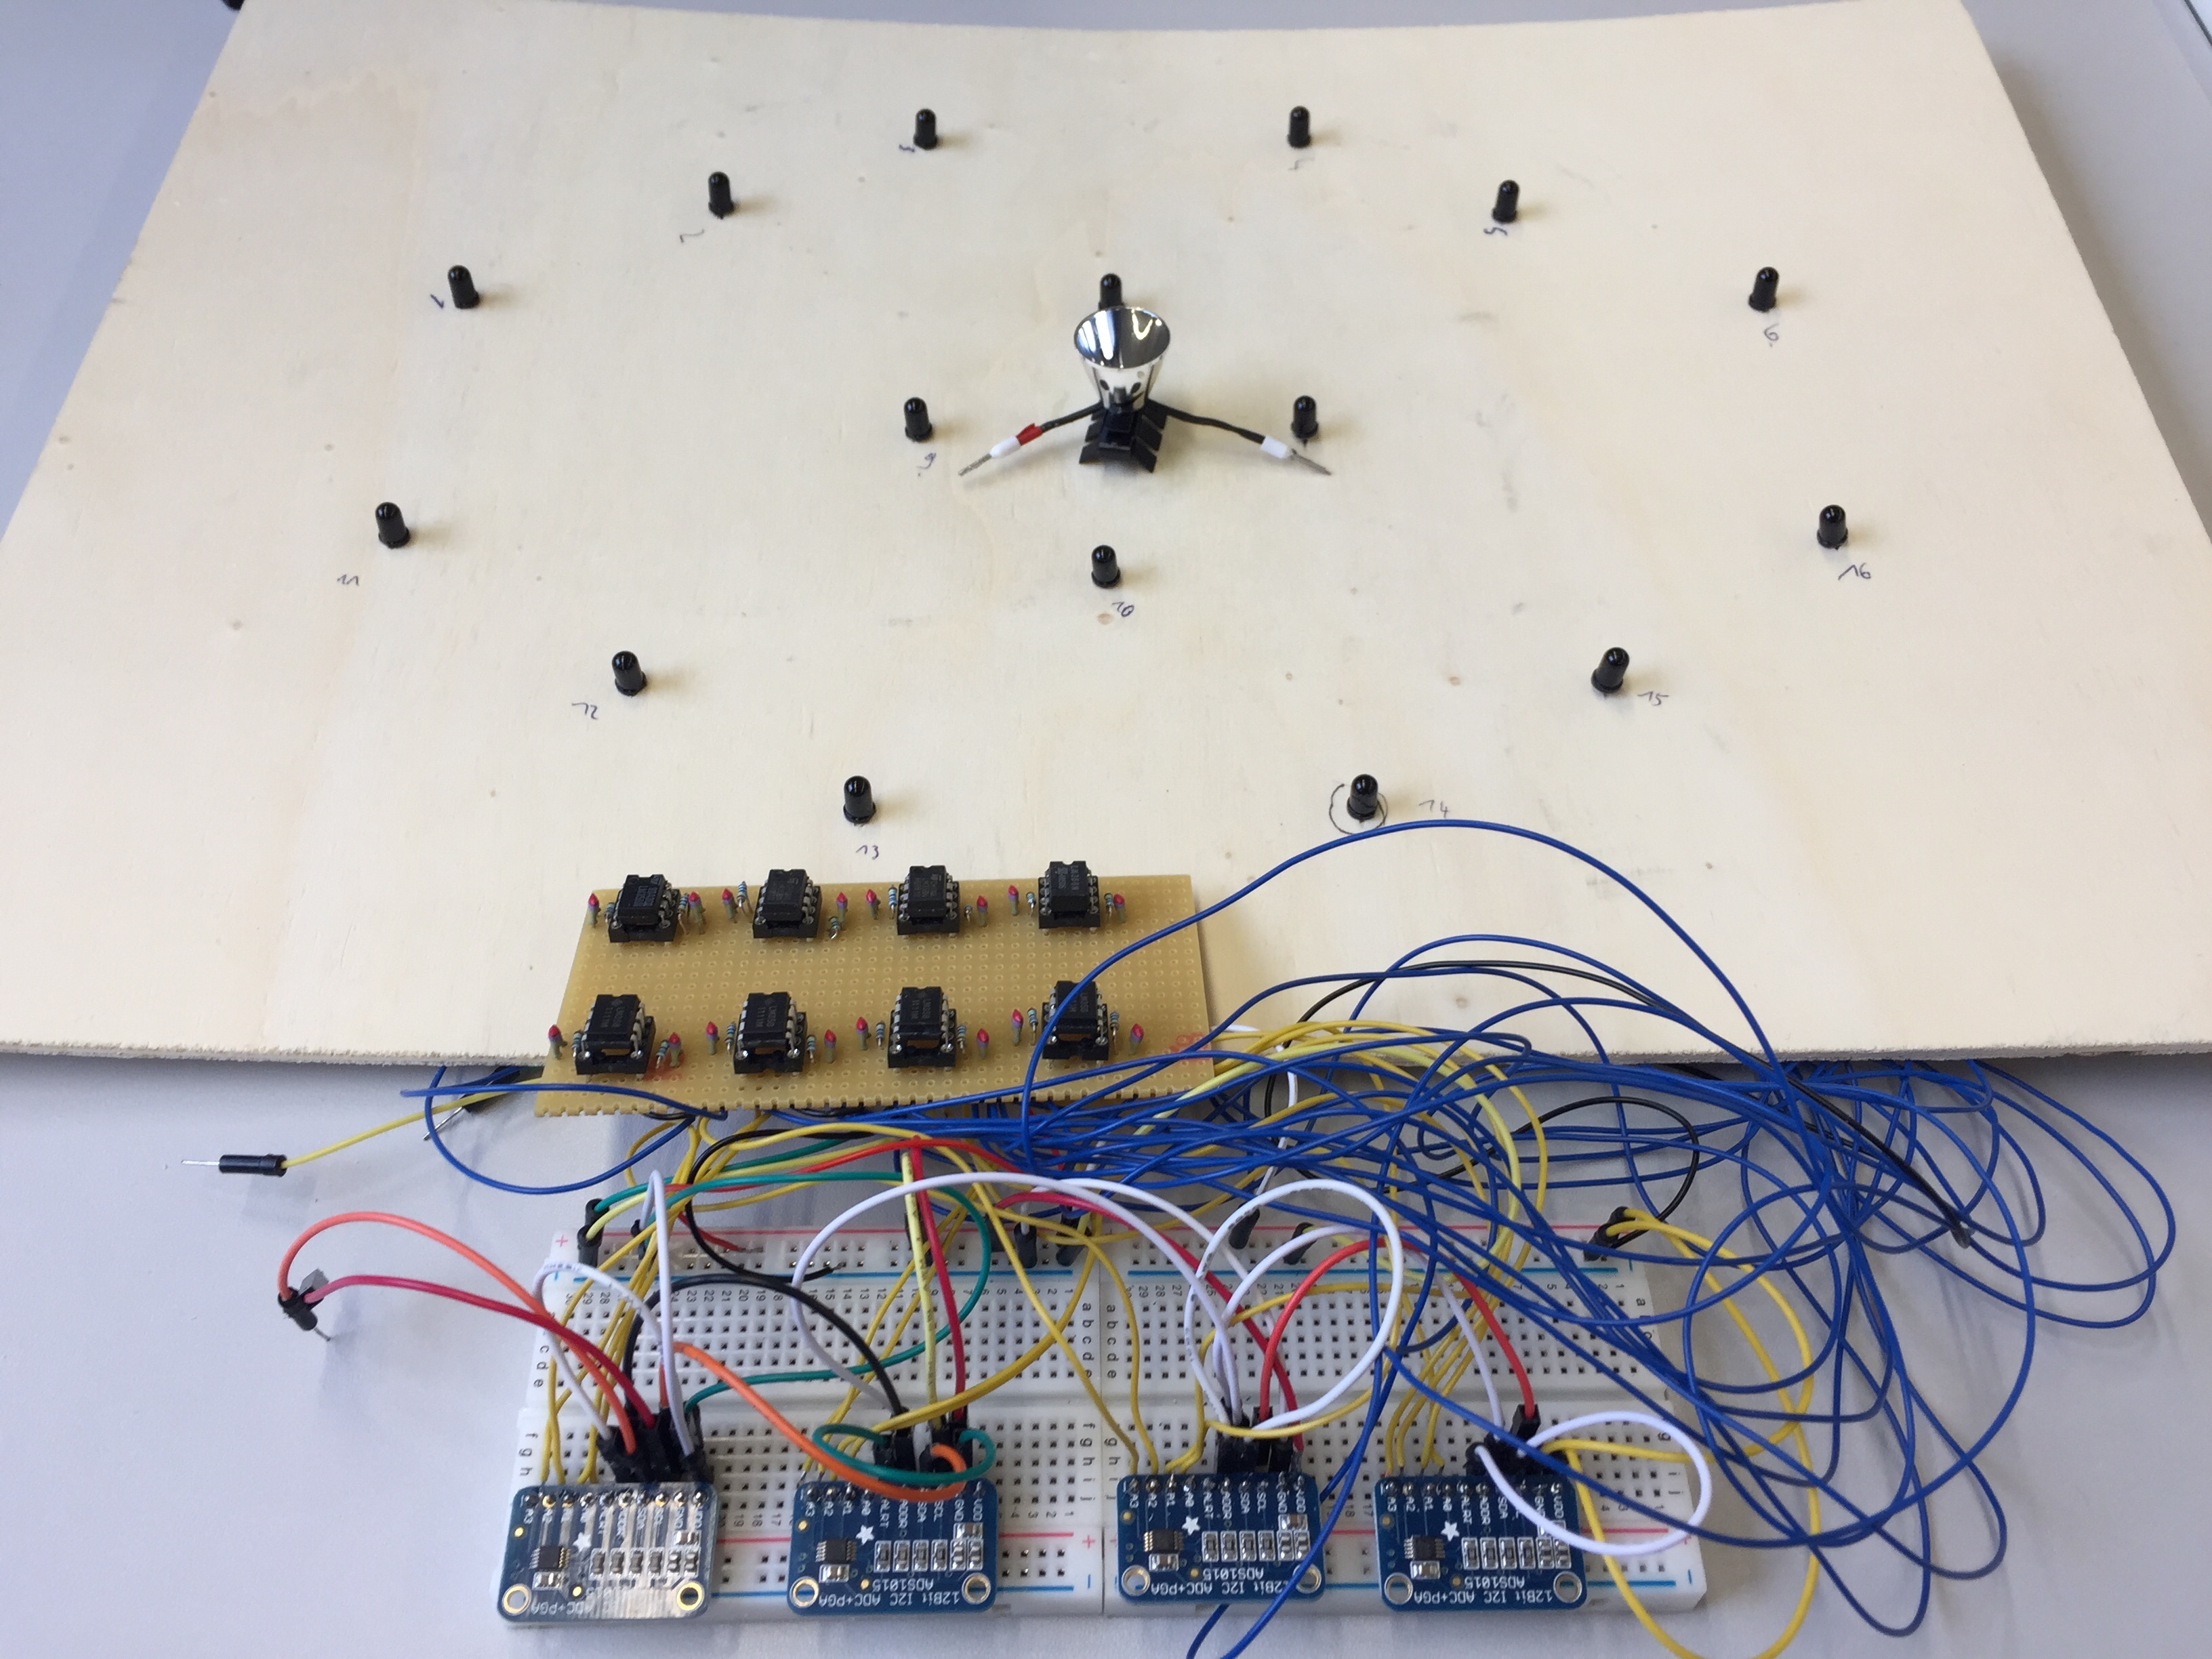
\includegraphics[scale=0.35]{figures/PhotoplatteBeta.jpeg}
	\caption{Beta-Verion der Photoplatte. Schwer zu transportieren und nicht modular!}
	\label{fig:Sensorhandschuh}
\end{figure}

Nun machten wir uns daran die Photoplatte transportabel und modularer zu gestalten. Dafür führten wir verschiedene Steckmodule ein, welche zu einer Photoplatte zusammengesteckt werden kann. 

%%% Introduction
\section{Photoplatte}
Die neue Photoplatte besteht aus zwei verschiedenen Teilen, einem Oktokommander als Herzstück der Photoplatte und passend dazu sieben Detektormodule. Die Detektormodule werden durch einen USB-Anschluss an den Oktokommander abgeschlossen. Ein freier Platz an den Oktokommander ist für die Verbindung zu der Software.

\begin{figure}[h]
	\centering
	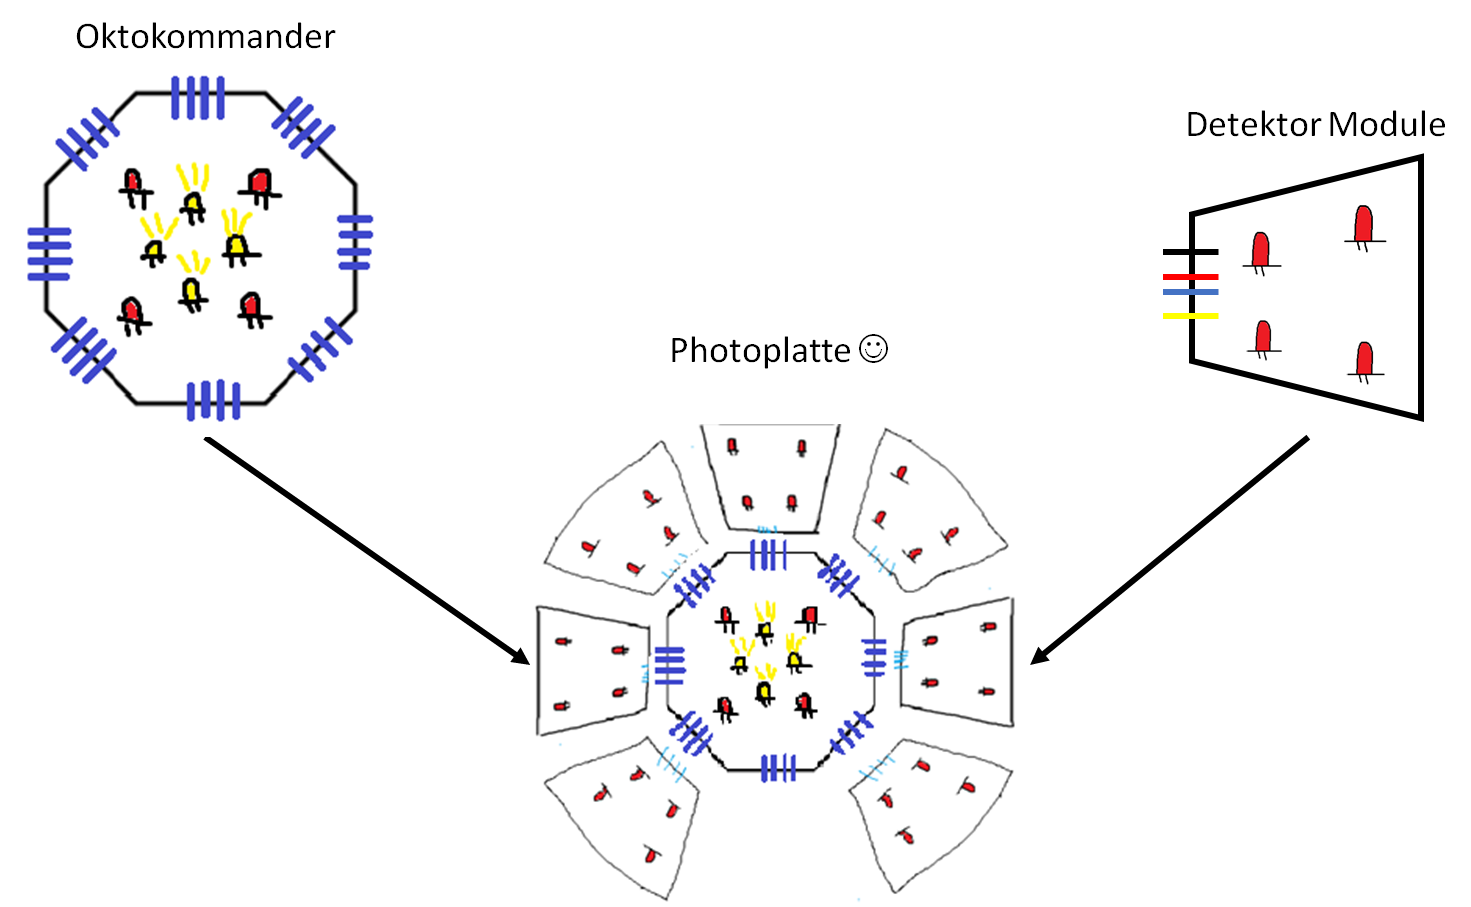
\includegraphics[scale=0.8]{figures/Photoplatte.png}
	\caption{Oktokommander und Detektormodule zusammen ergeben die neue modulare Photoplatte.}
	\label{fig:Sensorhandschuh}
\end{figure}

\section{Oktokommander}
Der Oktokommander ist das Steuersystem der gesamten Photoplatte. Sie besteht aus:
\begin{itemize}
\item Einem Arduino Micro
\item Einen i2c Expander
\item Einen i2c Multiplexer inklusive Verstärkerschaltung
\item Vier Photodioden
\item Vier infrarot LED Quellen
\item Sieben USB-Anschlüsse für die Detektormodule
\end{itemize}

\begin{figure}[h]
	\centering
	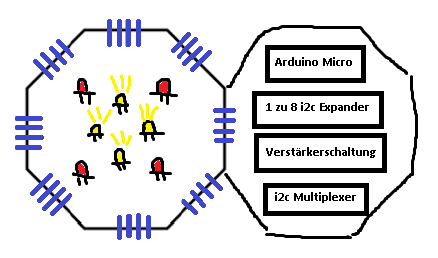
\includegraphics[scale=1.3]{figures/OktokommanderOffen.png}
	\caption{Oktokommander mit Blick auf alle Innenteile.}
	\label{fig:Sensorhandschuh}
\end{figure}

\section{Detektormodul}
Die Detektormodule bestehen aus jeweils vier Photodioden zur detektion der Lichtreflexionen der Hand. Sie werden durch den USB-Eingang an den Oktokommander angeschlossen. 

\begin{figure}[h]
	\centering
	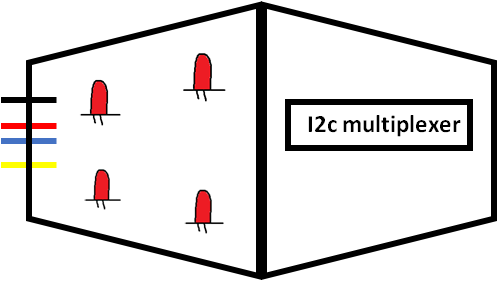
\includegraphics[scale=1.3]{figures/DetektormodulOffen.png}
	\caption{Oktokommander mit Blick auf alle Innenteile.}
	\label{fig:Sensorhandschuh}
\end{figure}

\section{Software}
\textcolor{red}{Hier kommt noch der Software Teil}

\section{Ausblick}
Als Ausblick unseres Gestikulaser wäre eine Verfeinerung der aktuell durchführbaren Gestenerkennung
denkbar, die nicht nur die Stellung der Hand, sondern auch die Krümmung der
einzelnen Finger berücksichtigt. Zu diesem Zweck wurde bereits ein Prototyp für einen
Sensorhandschuh entwickelt.

\begin{figure}[h]
	\centering
	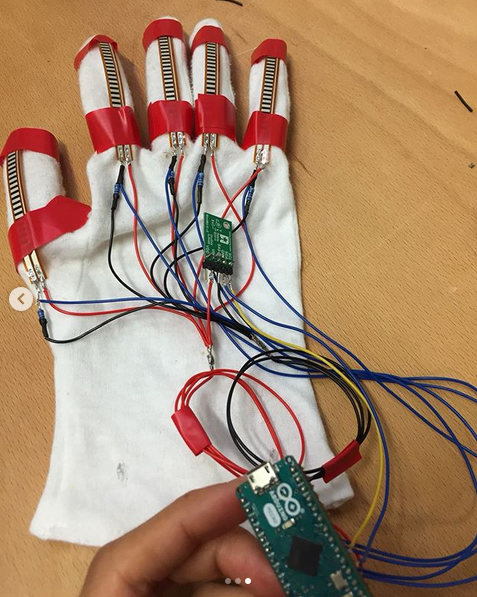
\includegraphics[scale=1.4]{figures/Sensorhandschuh}
	\caption{Aktueller Prototyp des Sensorhandschuhs. Es sind Biegesensoren für alle Finger, ein Gyroskop und ein Beschleunigungssensor im Einsatz. Bei der  
	Verarbeitung der Sensordaten kommt ein Arduino Micro zum Einsatz.}
	\label{fig:Sensorhandschuh}
\end{figure}

\section{Sponsoren}
Einen besonderen Dank gilt unseren Sponsoren: \\
\begin{tabularx}{\textwidth}{p{10cm} c}
	Aconity3D GmbH & \noindent\parbox[c]{\hsize}{
\includegraphics[scale=1]{Logos/aconity.png}} \\
	& \\
	Fraunhofer ILT & \noindent\parbox[c]{\hsize}{
\includegraphics[scale=1.2]{Logos/ILT.png}} \\
	& \\
	Würth Electronik GmbH \& Co. KG & \noindent\parbox[c]{\hsize}{
\includegraphics[scale=0.1]{Logos/Wuerth.png}}
\end{tabularx} \\

\end{multicols}

\conference{\raisebox{0.5cm}[0cm]{
\includegraphics[height=3cm]{Logos/VDE.jpg} } \hfill
\raisebox{1.25cm}[0cm]{
\includegraphics[height=1.5cm]{Logos/Faulhaber.png}} \hfill
\raisebox{0cm}[0cm]{
\includegraphics[height=4cm]{Logos/micronit.jpg}} \hfill
\raisebox{0cm}[0cm]{
\includegraphics[height=4cm]{Logos/electronica.png}} \hfill 
\raisebox{0cm}[0cm]{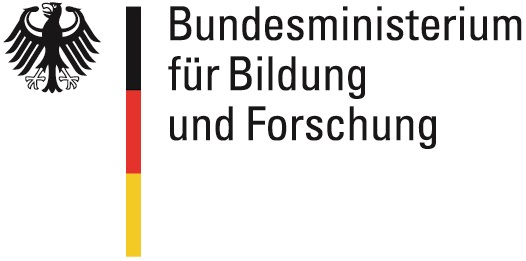
\includegraphics[height=4cm]{Logos/BMBF.jpg}}}

\end{document}